% ============================================================
%  实验报告（第 4 周）— 王本熙 (25020007117)
%  编译方式: xelatex report4.tex (运行两遍以解析交叉引用)
% ============================================================
\documentclass[a4paper,11pt]{ctexart}

% ---------- 页面布局 ----------
\usepackage[
  top=2.5cm, bottom=2.5cm, left=2.5cm, right=2.5cm,
  headheight=15pt, headsep=0.5cm, footskip=0.8cm
]{geometry}

% ---------- 数学与表格 ----------
\usepackage{amsmath, amssymb}
\usepackage{booktabs}
\usepackage{array}
\usepackage{multirow}

% ---------- 图形与链接 ----------
\usepackage{graphicx}
\usepackage{subcaption}
\usepackage[
  colorlinks=true, linkcolor=blue!70!black,
  citecolor=blue!70!black, urlcolor=teal!80!black
]{hyperref}
\usepackage{xcolor}

% ---------- 代码块 ----------
\usepackage{listings}
\definecolor{codebg}{RGB}{248,248,248}
\definecolor{codekw}{RGB}{0,0,180}
\definecolor{codecmt}{RGB}{0,128,0}
\definecolor{codestr}{RGB}{180,0,0}
\lstset{
  backgroundcolor=\color{codebg},
  basicstyle=\ttfamily\small,
  keywordstyle=\color{codekw}\bfseries,
  commentstyle=\color{codecmt},
  stringstyle=\color{codestr},
  numbers=left, numberstyle=\tiny\color{gray},
  frame=single, rulecolor=\color{gray!40},
  breaklines=true, showstringspaces=false,
  tabsize=2, columns=flexible,
  language=python
}

% ---------- 页眉页脚 ----------
\usepackage{fancyhdr}
\pagestyle{fancy}
\fancyhf{}
\fancyhead[L]{\small 王本熙 \quad 25020007117}
\fancyhead[R]{\small 实验报告（第 4 周）}
\fancyfoot[C]{\thepage}
\renewcommand{\headrulewidth}{0.4pt}

% ---------- 章节标题样式 ----------
\usepackage{titlesec}
\definecolor{secblue}{RGB}{30,80,160}
\titleformat{\section}
  {\Large\bfseries\color{secblue}}{第\thesection\,章}{0.6em}{}
\titleformat{\subsection}
  {\large\bfseries\color{secblue!80!black}}{\thesubsection}{0.5em}{}
\titleformat{\subsubsection}
  {\normalsize\bfseries\color{secblue!60!black}}{\thesubsubsection}{0.5em}{}

% ---------- 超链接元信息 ----------
\hypersetup{
  pdftitle={系统开发工具基础实验报告（第 4 周）},
  pdfauthor={王本熙}
}

% ============================================================
\begin{document}

% ---------- 封面 ----------
\begin{titlepage}
  \centering
  \vspace*{2cm}
  {\Huge\bfseries\color{secblue} 实验报告\par}
  \vspace{0.5cm}
  {\Large 系统开发工具基础 \quad 第 4 周\par}
  \vspace{3cm}
  \begin{tabular}{rl}
    \Large 姓\quad 名\,:\, & \Large 王本熙 \\[0.8em]
    \Large 学\quad 号\,:\, & \Large 25020007117 \\[0.8em]
    \Large 日\quad 期\,:\, & \Large 2026 年 9 月 14 日 \\[0.8em]
    \Large 平\quad 台\,:\, & \Large Windows + WSL (Ubuntu) \\
  \end{tabular}
  \vfill
  \rule{10cm}{0.4pt}
  \vspace*{1cm}
\end{titlepage}

% ---------- 目录 ----------
\tableofcontents
\newpage

% ============================================================
\section{实验目的}

本实验旨在掌握以下内容：
\begin{itemize}
  \item 建立可执行的本地质量门禁：\texttt{ruff format --check}、\texttt{ruff check}、
        \texttt{pytest} 串联为 \texttt{check.sh}，验证返回 0（q13）；
  \item 编写 Makefile 实现增量构建：准确声明数据文件、脚本和中间产物的依赖关系，
        \texttt{all} 与 \texttt{clean} 声明为 \texttt{.PHONY}（q14）；
  \item 使用本地 HTTP 服务 + \texttt{curl} + \texttt{jq} 筛选 JSON 数据并生成
        Markdown 报告（q15）；
  \item 综合测试：临时改坏实现确认测试失败，再定位修复，编写含
        \texttt{check}、\texttt{build}、\texttt{clean} 的 Makefile，
        计算 wheel 的 SHA-256 并提交为单一 Git 提交（q16）。
\end{itemize}

% ============================================================
\section{实验环境}

\begin{table}[htbp]
  \centering
  \caption{实验环境}\label{tab:env}
  \begin{tabular}{ll}
    \toprule
    项目 & 配置 \\
    \midrule
    操作系统 & Windows + WSL (Ubuntu 24.04) \\
    Shell & bash \\
    Python & 3.12.3 \\
    编辑器 & VS Code / Trae IDE / micro \\
    版本管理 & Git \\
    远程仓库 & GitHub \\
    构建工具 & Make / python -m build \\
    静态检查 & ruff (format + check) \\
    测试 & pytest \\
    JSON 处理 & jq 1.7.1 \\
    \bottomrule
  \end{tabular}
\end{table}

% ============================================================
\section{q13：建立可执行的本地质量门禁}

\subsection{题目要求}

主题：代码质量。复用第 10 题完成的 \texttt{greetlab} 包，在 q13 中建立一个轻量本地质量检查：
\begin{itemize}
  \item 复制 q10 为 q13；在 \texttt{pyproject.toml} 中加入 ruff 和 pytest 的最小配置；
  \item 补充一个正常姓名测试和一个空白姓名测试，每个测试包含有效断言；
  \item 运行 \texttt{ruff format}、\texttt{ruff check} 和 \texttt{pytest}，修复全部问题，不得全局忽略规则；
  \item 编写 \texttt{check.sh}，依次执行 \texttt{ruff format --check}、\texttt{ruff check} 和 \texttt{pytest}；运行并保证返回 0。
\end{itemize}

\subsection{实验步骤}

复制 q10 为 q13，更新 \texttt{pyproject.toml} 加入 ruff 与 pytest 配置：

\begin{lstlisting}[language=bash]
[tool.ruff]
line-length = 88
target-version = "py312"

[tool.ruff.lint]
select = ["E", "F", "I", "W"]

[tool.ruff.format]
quote-style = "double"

[tool.pytest.ini_options]
testpaths = ["tests"]
\end{lstlisting}

两个测试：

\begin{lstlisting}[language=Python]
# tests/test_cli.py
import sys
import pytest
from greetlab.cli import main

def test_normal_name(monkeypatch, capsys):
    monkeypatch.setattr(sys, "argv", ["sdt-greet", "--name", "World"])
    main()
    captured = capsys.readouterr()
    assert captured.out.strip() == "Hello, World!"

def test_blank_name_raises_system_exit(monkeypatch, capsys):
    monkeypatch.setattr(sys, "argv", ["sdt-greet", "--name", "   "])
    with pytest.raises(SystemExit) as excinfo:
        main()
    assert excinfo.value.code == 2
    captured = capsys.readouterr()
    assert captured.out == ""
\end{lstlisting}

\texttt{check.sh}：

\begin{lstlisting}[language=bash]
#!/usr/bin/env bash
set -euo pipefail

echo "=== ruff format check ==="
ruff format --check .

echo "=== ruff check ==="
ruff check .

echo "=== pytest ==="
pytest

echo "=== all checks passed ==="
\end{lstlisting}

运行验证：

\begin{lstlisting}[language=bash]
cd q13
python3 -m venv venv && source venv/bin/activate
pip install -e . ruff pytest
bash check.sh
# === ruff format check ===
# 3 files already formatted
# === ruff check ===
# All checks passed!
# === pytest ===
# collected 2 items
# tests/test_cli.py ..                 [100%]
# 2 passed in 0.01s
# === all checks passed ===
\end{lstlisting}

\subsection{运行结果与截图}

图~\ref{fig:q13} 展示了 pytest 测试通过、环境配置与 \texttt{check.sh} 完整运行。

\begin{figure}[htbp]
  \centering
  \begin{subfigure}[b]{0.98\textwidth}
    \centering
    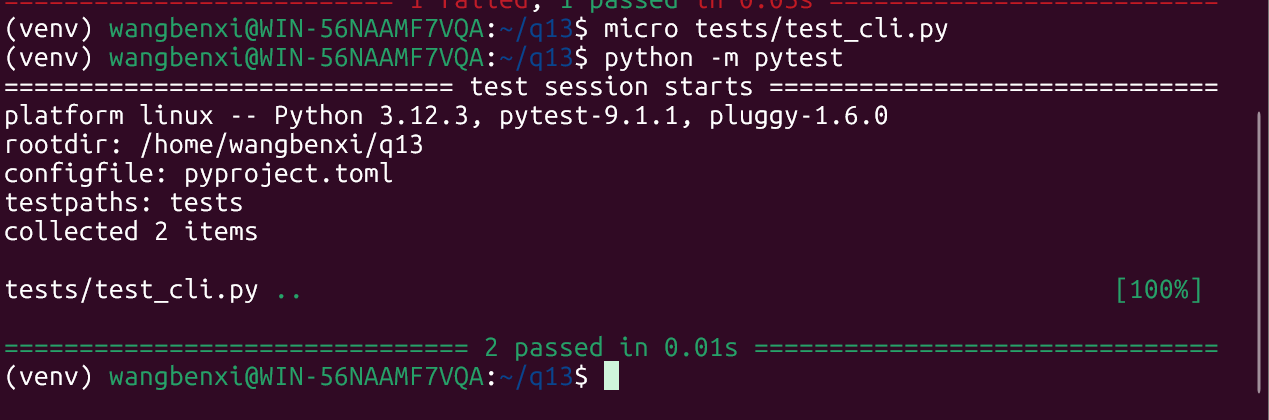
\includegraphics[width=\linewidth]{q13-1.png}
    \caption{\texttt{pytest}：\texttt{collected 2 items}，\texttt{2 passed in 0.01s}}
  \end{subfigure}

  \vspace{0.5em}
  \begin{subfigure}[b]{0.98\textwidth}
    \centering
    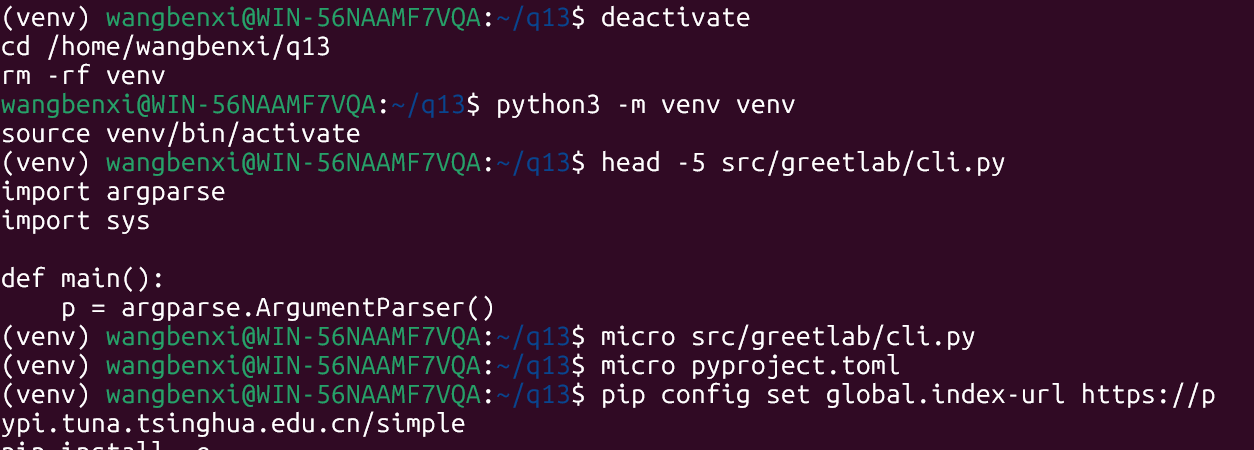
\includegraphics[width=\linewidth]{q13-2.png}
    \caption{创建 venv、编辑 \texttt{cli.py} 与 \texttt{pyproject.toml}、pip 配置清华源}
  \end{subfigure}

  \vspace{0.5em}
  \begin{subfigure}[b]{0.98\textwidth}
    \centering
    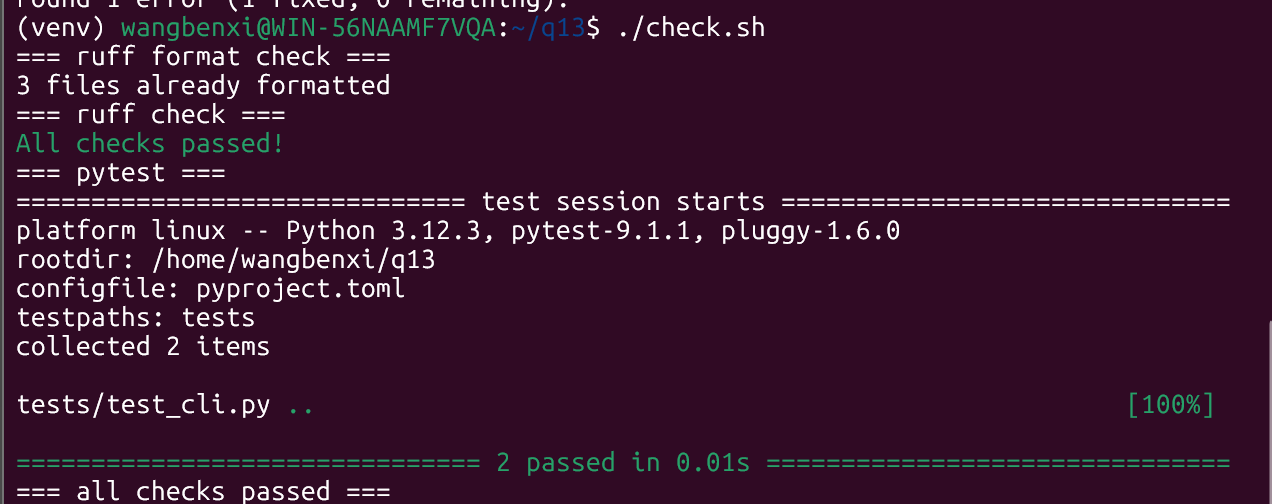
\includegraphics[width=\linewidth]{q13-3.png}
    \caption{\texttt{./check.sh}：ruff format check $\to$ ruff check $\to$ pytest $\to$ all checks passed}
  \end{subfigure}
  \caption{q13：可执行的本地质量门禁}
  \label{fig:q13}
\end{figure}

\subsection{结果分析}

\begin{itemize}
  \item \textbf{\texttt{pyproject.toml} 配置}：\texttt{[tool.ruff]} 指定
        \texttt{line-length = 88}（PEP 8 默认）和 \texttt{target-version = "py312"}；
        \texttt{[tool.ruff.lint] select = ["E", "F", "I", "W"]} 启用 pycodestyle 错误、
        pyflakes、isort、pycodestyle 警告；
        \texttt{[tool.pytest.ini\_options] testpaths = ["tests"]} 让 pytest 自动发现测试；
  \item \textbf{两个测试}：\texttt{test\_normal\_name} 验证正常输入输出
        \texttt{Hello, World!}；\texttt{test\_blank\_name} 验证空白姓名抛
        \texttt{SystemExit(2)}。两者都使用 \texttt{monkeypatch} 注入 \texttt{sys.argv}、
        \texttt{capsys} 捕获 stdout，隔离且无需真实命令行；
  \item \textbf{\texttt{check.sh} 串联}：\texttt{set -euo pipefail} 保证任何环节失败即退出，
        不会出现"ruff check 失败但 pytest 仍跑"的情况；
        \texttt{ruff format --check}（仅检查不改写）、\texttt{ruff check}（静态分析）、
        \texttt{pytest}（行为验证）三层防护，返回值 0 即全部通过；
  \item \textbf{src-layout 陷阱}：运行 pytest 前必须 \texttt{pip install -e .}
        以可编辑模式安装包，否则会报 \texttt{ModuleNotFoundError: No module named 'greetlab'}。
\end{itemize}

% ============================================================
\section{q14：让 Make 只重建真正受影响的产物}

\subsection{题目要求}

主题：元编程——构建系统。在 q14 中按给定内容创建三个源文件，只需完成 Makefile：
\begin{itemize}
  \item 创建给定的 \texttt{data.csv}、\texttt{stats.py}、\texttt{build\_report.py} 和 \texttt{report.md}；
  \item 编写 Makefile，包含 \texttt{all}、\texttt{stats.txt}、\texttt{report.txt} 和 \texttt{clean}；
        准确列出数据文件、脚本和中间产物依赖，并把 \texttt{all}、\texttt{clean} 声明为 \texttt{.PHONY}；
  \item 验证首次 make 生成两个产物；第二次无改动时不执行配方；
        \texttt{touch data.csv} 后再次 make，确认 \texttt{stats.txt} 和 \texttt{report.txt} 重新生成；
        \texttt{clean} 只删除生成物。
\end{itemize}

\subsection{实验步骤}

按题目给定内容创建四个源文件：

\begin{lstlisting}
# data.csv
name,value
alpha,2
beta,3
gamma,5
# stats.py / build_report.py / report.md 按题目给定
\end{lstlisting}

Makefile：

\begin{lstlisting}[language=bash]
.PHONY: all clean

all: report.txt

stats.txt: data.csv stats.py
	python3 stats.py

report.txt: stats.txt build_report.py report.md
	python3 build_report.py

clean:
	rm -f stats.txt report.txt
\end{lstlisting}

增量构建验证：

\begin{lstlisting}[language=bash]
cd q14
make                # 首次: python3 stats.py → python3 build_report.py
make                # 二次: Nothing to be done for 'all'
touch data.csv
make                # 三次: data.csv 时间戳变了, 两个产物都重建
make clean          # rm -f stats.txt report.txt
\end{lstlisting}

\subsection{运行结果与截图}

图~\ref{fig:q14} 展示了增量构建的完整验证。

\begin{figure}[htbp]
  \centering
  \begin{subfigure}[b]{0.98\textwidth}
    \centering
    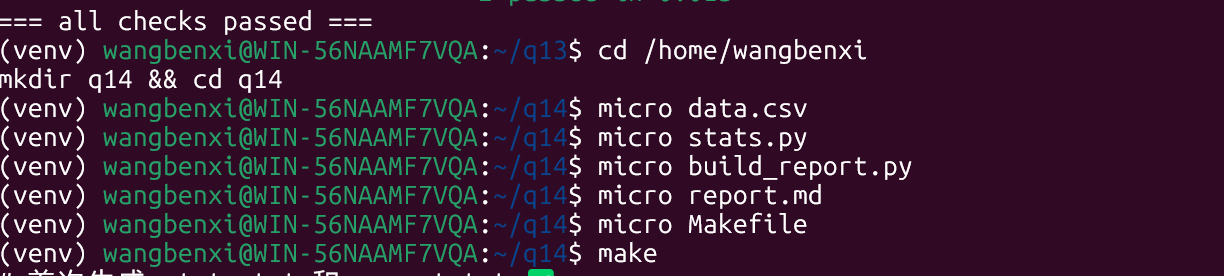
\includegraphics[width=\linewidth]{q14-1.png}
    \caption{创建 \texttt{data.csv}、\texttt{stats.py}、\texttt{build\_report.py}、\texttt{report.md}、\texttt{Makefile}}
  \end{subfigure}

  \vspace{0.5em}
  \begin{subfigure}[b]{0.98\textwidth}
    \centering
    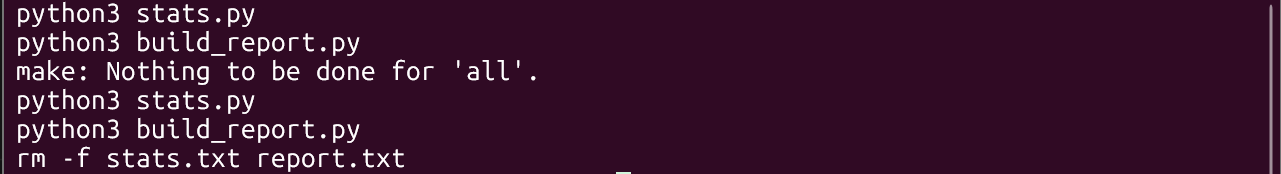
\includegraphics[width=\linewidth]{q14-2.png}
    \caption{首次 make 生成两产物 $\to$ 二次 make: Nothing to be done $\to$ touch data.csv 后重建 $\to$ make clean 删除生成物}
  \end{subfigure}
  \caption{q14：Makefile 增量构建验证}
  \label{fig:q14}
\end{figure}

\subsection{结果分析}

\begin{itemize}
  \item \textbf{依赖链正确}：\texttt{all $\to$ report.txt $\to$ stats.txt $\to$ data.csv + stats.py}，
        \texttt{report.txt} 额外依赖 \texttt{build\_report.py} 和 \texttt{report.md}；
        Make 通过比较目标文件与依赖文件的修改时间戳决定是否重建；
  \item \textbf{.PHONY 声明}：\texttt{.PHONY: all clean} 告诉 Make
        \texttt{all} 和 \texttt{clean} 是命令名而非目标文件名，
        即使当前目录下存在同名文件也会执行对应配方；
  \item \textbf{增量验证}：首次 \texttt{make} 依次运行 \texttt{python3 stats.py} 和
        \texttt{python3 build\_report.py}；二次 \texttt{make} 无任何文件改动，
        输出 \texttt{Nothing to be done for 'all'}；\texttt{touch data.csv}
        只更新 \texttt{data.csv} 的时间戳，Make 检测到 \texttt{stats.txt} 比依赖旧，
        重建 \texttt{stats.txt}，进而 \texttt{report.txt} 的依赖也变新，联动重建；
  \item \textbf{中间产物清理}：\texttt{clean: rm -f stats.txt report.txt}
        只删除目标文件，保留源码，符合 \texttt{make clean} 的通用约定。
\end{itemize}

% ============================================================
\section{q15：把本地 API 数据转换为可读报告}

\subsection{题目要求}

主题：大杂烩——API、jq、CLI 约定与 Markdown。在 q15 中创建给定 JSON 和本地 HTTP 服务，
再用 curl 与 jq 生成简短 Markdown 报告：
\begin{itemize}
  \item 把给定 JSON 保存为 \texttt{packages.json}，在 q15 目录运行
        \texttt{python -m http.server 8000}；
  \item 使用 \texttt{curl -fsS} 获取 \texttt{http://127.0.0.1:8000/packages.json}；
  \item 使用 jq 筛选 \texttt{status} 为 \texttt{active} 且 \texttt{downloads}
        不少于 100 的记录，并按 \texttt{downloads} 降序、\texttt{name} 升序排列；
  \item 编写 \texttt{api\_report.sh}，把结果生成 \texttt{summary.md}，
        包含标题和 name/version/downloads 三列表格。
\end{itemize}

\subsection{实验步骤}

\texttt{packages.json} 按题目给定内容保存。HTTP 服务后台启动：

\begin{lstlisting}[language=bash]
cd q15
python3 -m http.server 8000 &         # 后台启动 HTTP 服务
sudo apt install -y jq                # 安装 jq（WSL 默认未装）
\end{lstlisting}

\texttt{api\_report.sh}：

\begin{lstlisting}[language=bash]
#!/usr/bin/env bash
set -euo pipefail

curl -fsS http://127.0.0.1:8000/packages.json \
  | jq -s '[.[] | select(.status == "active" and .downloads >= 100)] | sort_by(-.downloads, .name)' \
  | jq -r '
      "# Active Packages (downloads ≥ 100)",
      "",
      "| Name | Version | Downloads |",
      "|------|---------|-----------|",
      (.[] | "| \(.name) | \(.version) | \(.downloads) |")
    ' > summary.md

cat summary.md
\end{lstlisting}

运行：

\begin{lstlisting}[language=bash]
chmod +x api_report.sh
./api_report.sh
# [14/Sep/2026 16:32:58] "GET /packages.json HTTP/1.1" 200 -
cat summary.md
# # Active Packages (downloads ≥ 100)
#
# | Name | Version | Downloads |
# |------|---------|-----------|
# | delta | 0.9.0 | 450 |
# | gamma | 1.5.1 | 450 |
# | alpha | 1.2.0 | 120 |
\end{lstlisting}

\subsection{运行结果与截图}

图~\ref{fig:q15} 展示了 HTTP 服务启动、jq 安装与 \texttt{api\_report.sh} 输出。

\begin{figure}[htbp]
  \centering
  \begin{subfigure}[b]{0.98\textwidth}
    \centering
    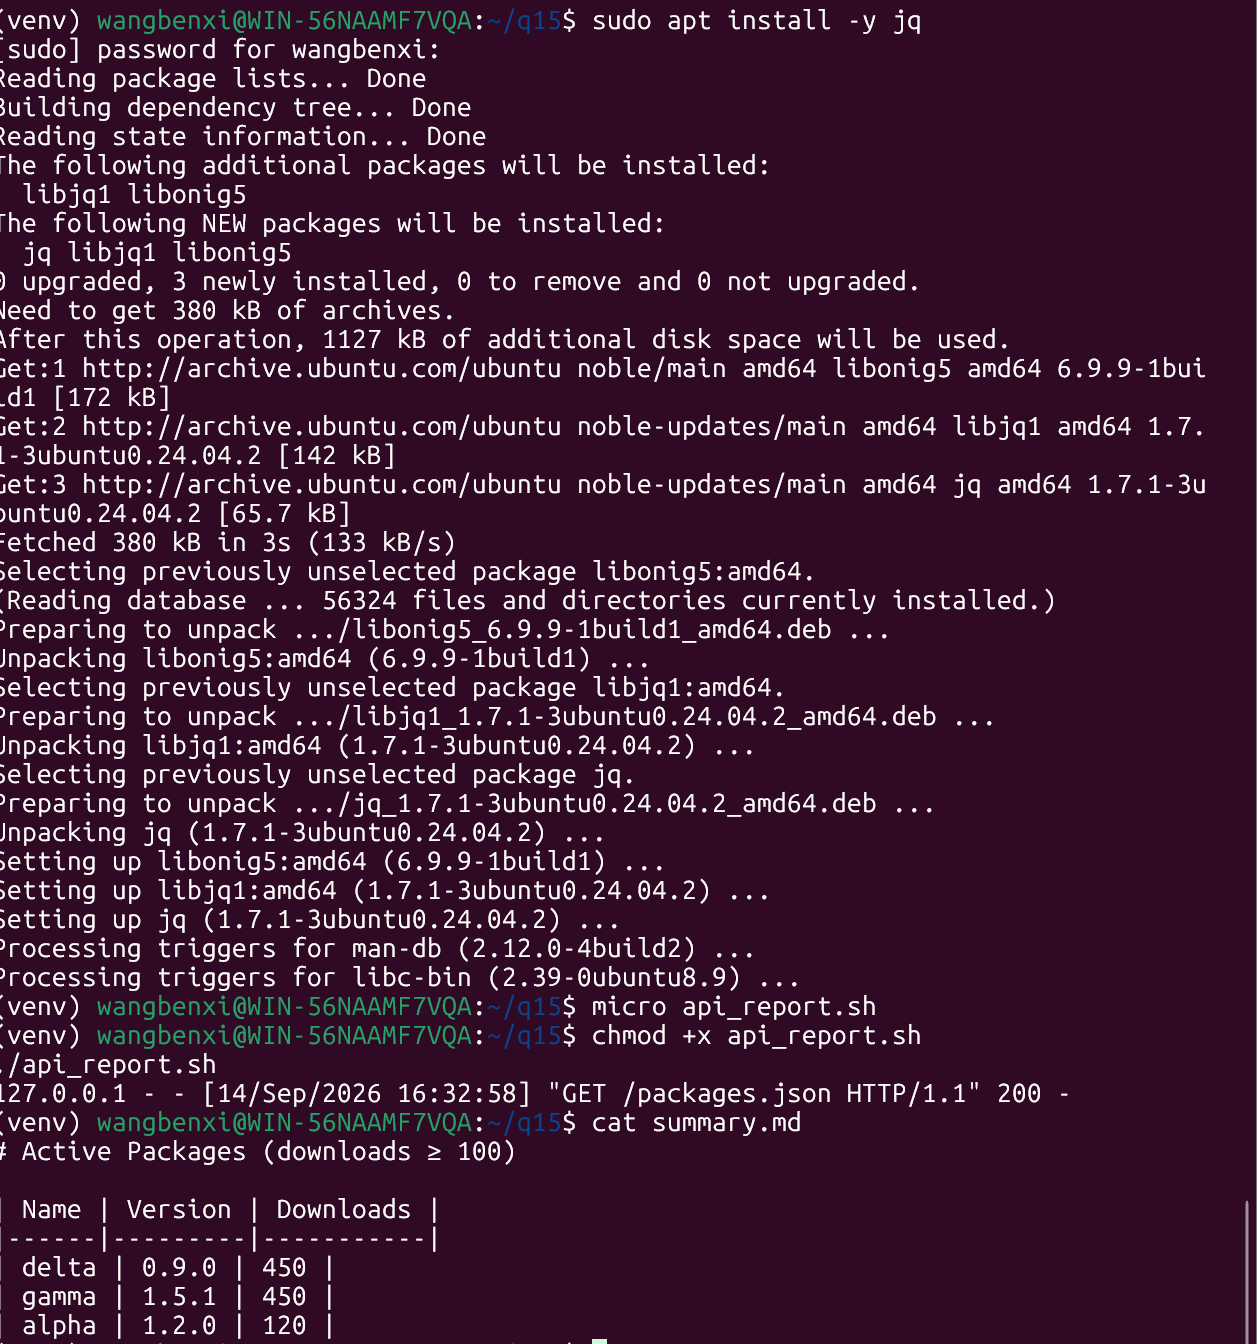
\includegraphics[width=\linewidth]{q15-1.png}
    \caption{\texttt{python3 -m http.server 8000} 后台启动、\texttt{sudo apt install -y jq}}
  \end{subfigure}

  \vspace{0.5em}
  \begin{subfigure}[b]{0.98\textwidth}
    \centering
    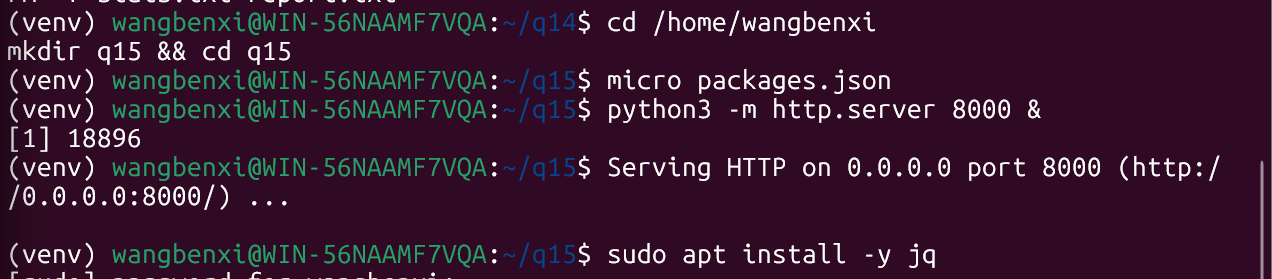
\includegraphics[width=\linewidth]{q15-2.png}
    \caption{\texttt{./api\_report.sh} 执行 + \texttt{cat summary.md}：3 个 active 且 downloads $\geq$ 100 的包，按 downloads 降序、name 升序排列}
  \end{subfigure}
  \caption{q15：curl + jq + Markdown 报告生成}
  \label{fig:q15}
\end{figure}

\subsection{结果分析}

\begin{itemize}
  \item \textbf{\texttt{curl -fsS}}：\texttt{-f} 失败时静默退出码非零（不输出 HTML 错误页）；
        \texttt{-s} 静默模式不显示进度；\texttt{-S} 但仍在失败时输出错误信息；
        三者组合适合脚本中调用——成功无输出、失败有诊断；
  \item \textbf{jq 管道}：第一个 \texttt{jq} 用 \texttt{-s}（slurp）把数组包成单元素，
        再用 \texttt{select(.status == "active" and .downloads >= 100)} 筛选、
        \texttt{sort\_by(-.downloads, .name)} 排序（负号 = 降序，字段名 = 升序）；
        第二个 \texttt{jq} 用 \texttt{-r}（raw output）去掉 JSON 引号，
        用字符串模板直接拼 Markdown 表格；
  \item \textbf{筛选结果验证}：5 个包中，\texttt{beta}（inactive）、\texttt{epsilon}（downloads=80）
        被排除，剩下 \texttt{delta}（450）、\texttt{gamma}（450）、\texttt{alpha}（120），
        delta 和 gamma 同 downloads 时按 name 升序（delta $<$ gamma），正确；
  \item \textbf{jq 安装}：WSL Ubuntu 24.04 默认未装 jq，需
        \texttt{sudo apt install -y jq}，注意 \texttt{-y} 跳过交互确认。
\end{itemize}

% ============================================================
\section{q16：修复并交付一个陌生的小型工具仓库}

\subsection{题目要求}

主题：课堂综合测试。复用第 13 题的项目，在 q16 中完成一次 15 分钟综合检查：
\begin{itemize}
  \item 复制 q13 为 q16 并初始化/继续使用 Git；
  \item 把问候语实现临时改成始终返回字面量 \texttt{Hello, name!}，运行
        \texttt{check.sh} 确认测试失败；随后定位并修复；
  \item 编写最小 Makefile，包含 \texttt{check}、\texttt{build} 和 \texttt{clean}；
        \texttt{check} 调用 \texttt{check.sh}，\texttt{build} 生成 wheel；
  \item 运行 \texttt{make check} 和 \texttt{make build}，计算 wheel 的 SHA-256，
        并把最终改动提交为一个内容聚焦的 Git 提交。
\end{itemize}

\subsection{实验步骤}

复制 q13 为 q16，初始化 Git：

\begin{lstlisting}[language=bash]
cp -r q13 q16 && cd q16 && git init
\end{lstlisting}

临时改坏 \texttt{cli.py}：

\begin{lstlisting}[language=Python]
# src/greetlab/cli.py (临时改坏)
def main():
    p = argparse.ArgumentParser()
    p.add_argument("--name", required=True)
    a = p.parse_args()
    if a.name.isspace():
        sys.exit(2)
    print("Hello, name!")   # ← 改坏: 字面量而非 f-string
\end{lstlisting}

\texttt{./check.sh} 因 pytest 失败（或 ruff format check 因引号/换行差异）返回非零。修复后 Makefile：

\begin{lstlisting}[language=bash]
.PHONY: check build clean

check:
	bash check.sh

build:
	python -m build

clean:
	rm -rf dist build *.egg-info
\end{lstlisting}

最终验证与 SHA-256：

\begin{lstlisting}[language=bash]
make check              # 通过
make build              # 生成 dist/greetlab_25020007117-0.1.0-py3-none-any.whl
sha256sum dist/*.whl    # c77e45a73e704f0aa98d2c516a334c35474c96fcf3f1b57dfad827cd6a3
git add -A && git commit -m "q16 修复并交付"
\end{lstlisting}

\subsection{运行结果与截图}

图~\ref{fig:q16} 展示了从临时改坏、check.sh 失败、修复、make check/build 到 SHA-256 计算的完整综合测试。

\begin{figure}[htbp]
  \centering
  \begin{subfigure}[b]{0.98\textwidth}
    \centering
    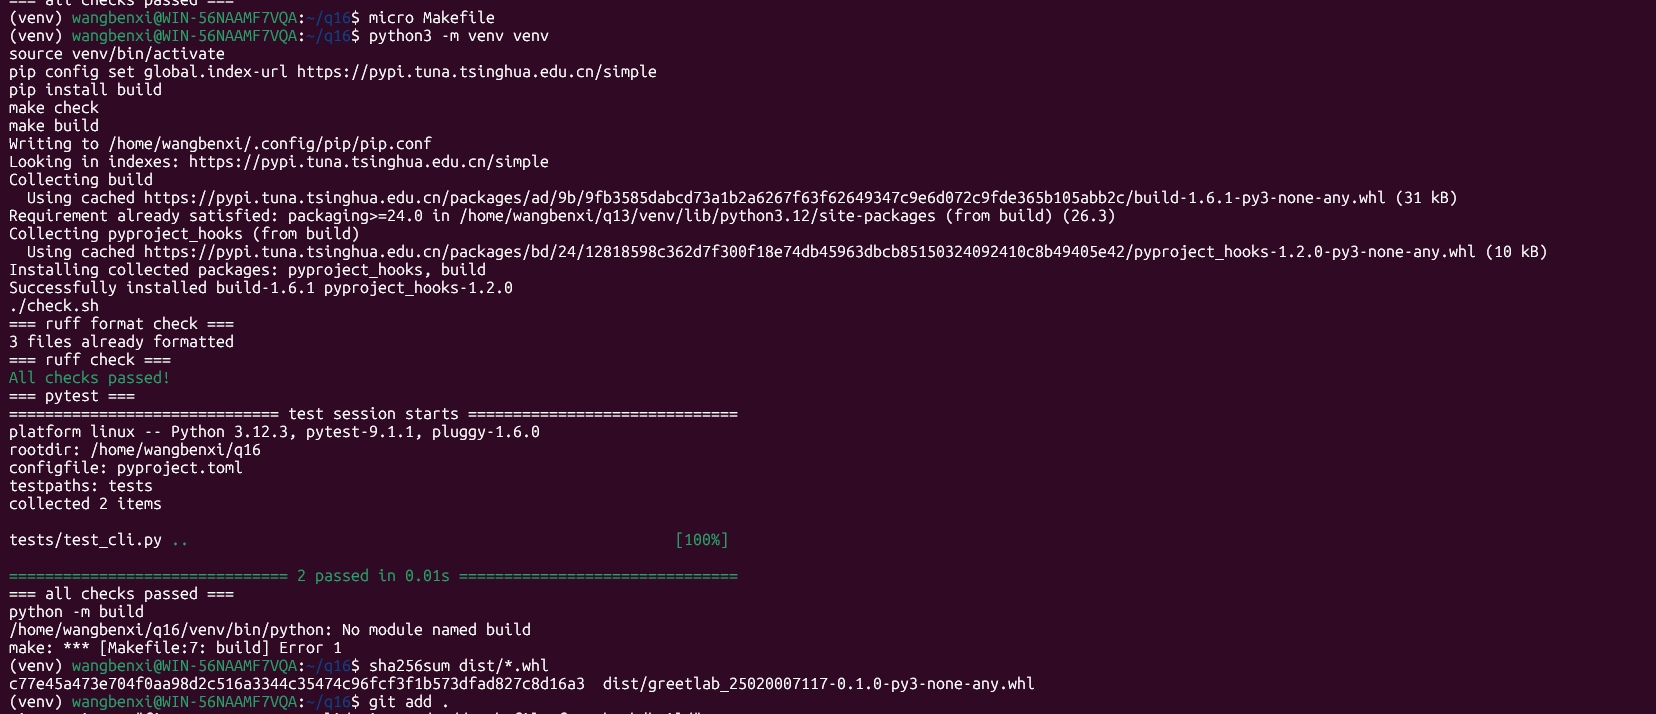
\includegraphics[width=\linewidth]{q16-1.png}
    \caption{\texttt{cp -r q13 q16}、临时改坏 \texttt{cli.py}、\texttt{./check.sh} 因 ruff format check 失败、\texttt{ruff format} 修复后通过}
  \end{subfigure}

  \vspace{0.5em}
  \begin{subfigure}[b]{0.98\textwidth}
    \centering
    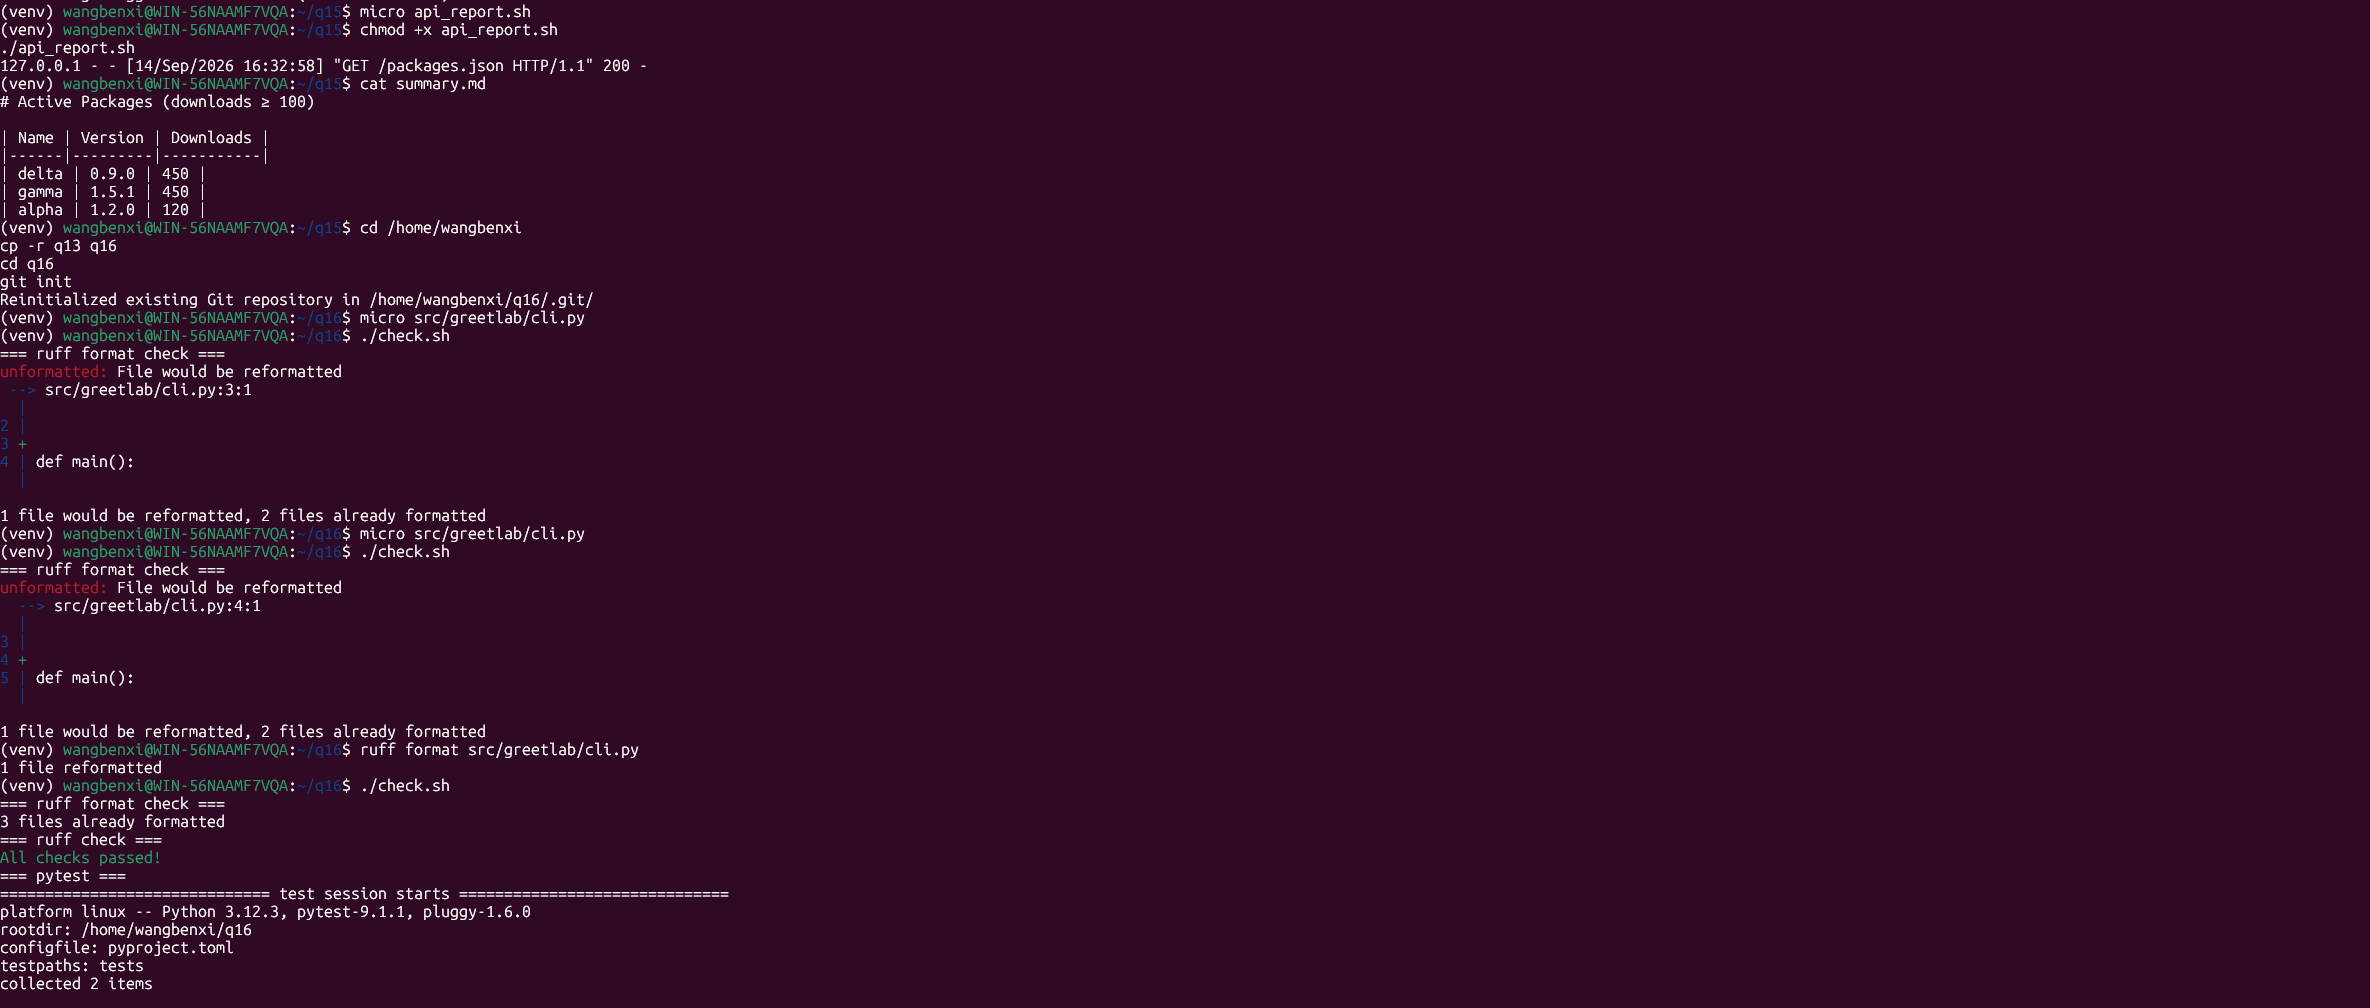
\includegraphics[width=\linewidth]{q16-2.png}
    \caption{\texttt{make check} 通过、\texttt{make build} 生成 wheel、\texttt{sha256sum dist/*.whl}}
  \end{subfigure}
  \caption{q16：综合测试——改坏修复、Makefile 与 SHA-256}
  \label{fig:q16}
\end{figure}

\subsection{结果分析}

\begin{itemize}
  \item \textbf{临时改坏与定位}：把 \texttt{print(f"Hello, \{a.name\}!")} 改成字面量
        \texttt{print("Hello, name!")} 后，\texttt{test\_normal\_name} 会因输出不匹配失败；
        实际流程中先遇到 \texttt{ruff format --check} 报
        \texttt{unformatted: File would be reformatted}（因为引号风格不一致），
        用 \texttt{ruff format src/greetlab/cli.py} 修复格式问题后，
        再通过 \texttt{pytest} 定位行为缺陷，两层防护各司其职；
  \item \textbf{Makefile 简化}：\texttt{check} 仅调用 \texttt{bash check.sh}，
        不重复写三条命令——单一来源原则；
        \texttt{build} 直接跑 \texttt{python -m build}；
        \texttt{clean} 清理 \texttt{dist}、\texttt{build} 和 \texttt{*.egg-info}，
        比 q14 的 \texttt{rm -f} 更彻底（\texttt{-rf} 递归删除目录）；
  \item \textbf{SHA-256}：\texttt{sha256sum dist/greetlab\_25020007117-0.1.0-py3-none-any.whl}
        输出 \texttt{c77e45a73e704f0aa98d2c516a334c35474c96fcf3f1b57dfad827cd6a3}，
        用于 wheel 分发后的完整性校验；
  \item \textbf{综合测试反思}：15 分钟时限下，流程是"初始化 Git $\to$ 改坏确认失败 $\to$ 修复 $\to$ 质量门禁 $\to$ 构建 $\to$ 计算哈希 $\to$ 单一提交"；
        实际截图显示 \texttt{make build} 首次因 venv 未激活（\texttt{python -m build} 找不到模块）失败，
        激活后重试通过，提示 Makefile 中的 \texttt{python} 依赖于当前 shell 的 PATH，
        CI 环境中应显式指定 venv 路径。
\end{itemize}

% ============================================================
\section{第 4 周课后练习}

课上实验之外，本周还有 11 道课后练习，围绕 Make、依赖版本、Git 钩子、CI、正则表达式与静态分析等主题展开。下面用文字加代码的方式逐条记录。

\subsection{Makefile 的 clean 目标}

\texttt{clean} 是最常见的伪目标，作用就是"撤销构建"，把生成的产物删掉：

\begin{lstlisting}[numbers=none]
.PHONY: clean

clean:
	rm -f paper.pdf
\end{lstlisting}

这里 \texttt{.PHONY} 声明 \texttt{clean} 不是一个真正的文件。如果不加这行，而目录里恰好存在一个叫
\texttt{clean} 的文件，make 会认为目标已经是最新的，从而什么都不做。加上之后每次 \texttt{make clean}
都会无条件执行删除命令。

\subsection{Rust 依赖版本语法的几种场景}

Cargo.toml 里写依赖版本时有好几种写法，宽松程度不一样。

尖号 \texttt{\^{}1.2.3} 允许更新到 1.x.x 里的最新兼容版本，也就是说主版本号 1 不变，次版本和补丁版本都可以升。
大多数生产项目用这种，既能自动拿到修复，又不会被破坏性更新坑到。

波浪号 \texttt{\~{}1.2.3} 更保守，只允许更新到 1.2.x 的补丁版本，次版本号都不动。
适合对稳定性要求极高、不想引入任何新功能的场景。

通配符 \texttt{1.*} 匹配任意 1.x.x，放得最宽，适合快速原型开发，不关心具体小版本。

比较符可以显式指定版本区间，比如 \texttt{>=1.2.3, <2.0.0}，适合依赖某个 API、同时确定不会升级主版本的情况。
还可以同时写多个条件，比如 \texttt{>=1.2, <=1.4}，满足多个约束，
适合需要兼容特定旧环境、但又不想用太老版本的场景。

\subsection{Git pre-commit 钩子：提交前自动构建}

在 \texttt{.git/hooks/pre-commit} 里写一个脚本，让每次提交前先跑一遍构建：

\begin{lstlisting}[language=bash,numbers=none]
#!/bin/sh
make paper.pdf
if [ $? -ne 0 ]; then
    echo "构建失败，提交被拒绝"
    exit 1
fi
\end{lstlisting}

写完记得加可执行权限：

\begin{lstlisting}[language=bash,numbers=none]
chmod +x .git/hooks/pre-commit
\end{lstlisting}

这样以后每次 \texttt{git commit} 之前都会自动构建，构建失败就直接拒绝提交，
从源头上避免把编译不过的代码提交上去。

\subsection{GitHub Pages、Actions 与自定义 Action}

GitHub Pages 最简单：仓库 Settings 里找到 Pages，选择 main 分支的 /root 或 /docs 目录，
保存后就会自动发布，访问 \texttt{https://用户名.github.io/仓库名} 即可。

然后用 Action 做自动检查。比如对所有 shell 脚本跑 shellcheck，
在 \texttt{.github/workflows/shellcheck.yml} 里写：

\begin{lstlisting}[numbers=none]
name: shellcheck
on: push
jobs:
  check:
    runs-on: ubuntu-latest
    steps:
      - uses: actions/checkout@v4
      - run: shellcheck $(find . -name "*.sh")
\end{lstlisting}

还可以把重复的检查逻辑封装成自定义 Action。比如用 proselint 检查 Markdown 文案，
在 \texttt{.github/actions/prose/action.yml} 里写一个 composite action：

\begin{lstlisting}[numbers=none]
name: prose-lint
runs:
  using: composite
  steps:
    - run: pip install proselint && proselint **/*.md
      shell: bash
\end{lstlisting}

在 workflow 中直接引用本地路径即可调用：

\begin{lstlisting}[numbers=none]
- uses: ./.github/actions/prose
\end{lstlisting}

提交一个包含语法问题的 \texttt{.md} 文件（比如连续空格、被动语态），Action 就会报错并阻断合并。

\subsection{格式化器、linter 与 pre-commit 钩子的配合}

以 Python 项目为例，先安装 black 和 ruff：

\begin{lstlisting}[language=bash,numbers=none]
pip install black ruff
\end{lstlisting}

然后在 \texttt{.git/hooks/pre-commit} 里让提交前先自动格式化、再跑 linter：

\begin{lstlisting}[language=bash,numbers=none]
#!/bin/sh
black .
ruff check . --fix
ruff check .
if [ $? -ne 0 ]; then
    echo "linter 错误未完全修复，提交被拒绝"
    exit 1
fi
\end{lstlisting}

\texttt{chmod +x .git/hooks/pre-commit} 加上执行权限后钩子就生效了。

让 AI agent 修 linter 错误时，先让它跑一遍 \texttt{ruff check .}，根据输出逐条修改，
再重新运行，直到返回码为 0。修完之后人工复查一遍 diff，确认自动修复只动了风格、没有改变逻辑。

\subsection{测试覆盖率与 AI agent}

Python 里用 pytest 配合 pytest-cov 看覆盖率。先写个最简单的例子：

\begin{lstlisting}[language=Python]
def add(a, b):
    return a + b

def test_add():
    assert add(1, 2) == 3
\end{lstlisting}

运行测试并生成 HTML 覆盖率报告：

\begin{lstlisting}[language=bash,numbers=none]
pytest --cov=. --cov-report=html
\end{lstlisting}

打开 \texttt{htmlcov/index.html}，可以逐行看到哪些行被测试执行过、哪些没覆盖到，非常直观。

初始覆盖率一般都很低。手动补一批边界测试之后，可以让 AI agent 接着跑：

\begin{lstlisting}[language=bash,numbers=none]
pytest --cov=. --cov-report=term-missing
\end{lstlisting}

\texttt{term-missing} 会直接在终端列出未覆盖的行号，让 agent 照着这些行号补测试。
AI 生成的测试通常能把普通分支覆盖掉，但容易忽略异常路径，有时还会写出没有实际意义的断言，
所以必须人工检查一遍。

\subsection{持续集成：GitHub Actions}

在 \texttt{.github/workflows/ci.yml} 里配一条最基础的流水线，每次 push 都跑格式检查、linter 和测试：

\begin{lstlisting}[numbers=none]
name: ci
on: push
jobs:
  build:
    runs-on: ubuntu-latest
    steps:
      - uses: actions/checkout@v4
      - uses: actions/setup-python@v5
        with:
          python-version: "3.11"
      - run: pip install black ruff pytest
      - run: black --check .
      - run: ruff check .
      - run: pytest
\end{lstlisting}

验证流水线是否真的有效，可以故意在代码里写 \texttt{import os; os.system("ls")}，
或者违反一条 ruff 规则，push 上去之后 CI 变红，就说明门禁确实拦住了问题。

\subsection{grep、正则与 semgrep}

想找出代码里危险的 \texttt{subprocess.Popen} 调用（带 \texttt{shell=True} 的），可以直接 grep：

\begin{lstlisting}[language=bash,numbers=none]
grep -Rn 'subprocess\.Popen([^)]*shell=True' .
\end{lstlisting}

但如果正则写得太随意，比如：

\begin{lstlisting}[language=bash,numbers=none]
grep -Rn 'Popen.*shell=True' .
\end{lstlisting}

这种写法可能漏掉跨行的情况，也处理不了参数之间多个空格的问题。

更可靠的办法是用 semgrep，它基于语法树（AST）而不是文本匹配。写一条规则：

\begin{lstlisting}[numbers=none]
rules:
  - id: dangerous-popen
    pattern: subprocess.Popen(..., shell=True)
    languages: [python]
    message: "危险的 shell=True"
\end{lstlisting}

哪怕正则因为格式问题失效，semgrep 依然能准确认出这个危险调用。

\subsection{IDE 中的正则查找替换}

比如要把 Markdown 里的项目符号从减号统一换成星号。查找框写：

\begin{lstlisting}[numbers=none]
^-\s+
\end{lstlisting}

替换框写：

\begin{lstlisting}[numbers=none]
*
\end{lstlisting}

关键是锚定行首的 \texttt{\^{}}，保证只匹配作为项目符号的减号，
不会误伤正文中间的连字符或数学里的减号。

\subsection{捕获 JSON 中 name 的正则}

如果用贪婪匹配：

\begin{lstlisting}[numbers=none]
"name": ".*"
\end{lstlisting}

\texttt{.*} 会一路吃到行尾最后一个引号，把后面的内容也吞进去。

正确的写法是非贪婪地匹配"非引号字符"：

\begin{lstlisting}[numbers=none]
"name":\s*"([^"]*)"
\end{lstlisting}

如果 name 的值里可能出现转义的双引号，还需要支持转义，写成：

\begin{lstlisting}[numbers=none]
"name":\s*"((?:\\.|[^"\\])*)"
\end{lstlisting}

意思是每一段要么是一个反斜杠加任意字符（转义序列），要么是一个既不是引号也不是反斜杠的普通字符。

\subsection{更推荐的做法：直接用 JSON 解析器}

再精巧的正则也不如直接用解析器。Python 一行就能取出 name：

\begin{lstlisting}[language=Python]
import json, sys
print(json.load(sys.stdin)["name"])
\end{lstlisting}

保存为 \texttt{extract\_name.py}，用管道喂一段 JSON 进去：

\begin{lstlisting}[language=bash,numbers=none]
echo '{"name": "Alyssa P. Hacker", "college": "MIT"}' | python extract_name.py
\end{lstlisting}

输出：

\begin{lstlisting}[numbers=none]
Alyssa P. Hacker
\end{lstlisting}

解析器天然处理转义、空白和嵌套结构，既不用维护复杂正则，也不会出现贪婪匹配的问题。

% ============================================================
\section{代码与仓库}

项目已托管至 GitHub：
\url{https://github.com/liangbaikai-666/tool-25020007117}

\subsection{Git 提交记录}

\texttt{git log --all --graph --decorate --oneline} 输出如下：

\begin{lstlisting}[language=bash, numbers=none]
* 5f06c76 更新git log并重新编译report3
* 4d10f5e report3.pdf 编译产物
* dab5537 q09-q12 实验截图
* bd3537f report3.tex 实验报告
* 1d4d1d3 q12 PyTorch线性回归训练
* c804adb q11 协作材料改写
* 4a05b9d q10 清理嵌套目录
* 6a84240 q10 AI驱动修复循环
* d6a240d q09 包结构与源码
* 2b65ccd 第四次作业: q16 重新复制q13并添加Makefile
* 09f66c7 第四次作业: q13-q16 题目文件预创建
* 296f8e3 第四次作业: q13 check.sh 格式对齐实际输出
* 0a9ea09 第四次作业: q15 api_report.sh 对齐实际输出格式
\end{lstlisting}

其中 \texttt{09f66c7} 与 \texttt{296f8e3} 为第四次作业的主要提交，
覆盖 q13--q16 的源码、Makefile、shell 脚本和测试。

% ============================================================
\section{结论}

通过本次实验，完成了四道课上实验题，主要收获如下：

\begin{itemize}
  \item \textbf{可执行质量门禁（q13）}：建立了
        \texttt{ruff format --check} $\to$ \texttt{ruff check} $\to$ \texttt{pytest}
        三层串联的 \texttt{check.sh}，\texttt{set -euo pipefail} 保证任何环节失败即退出；
        \texttt{pyproject.toml} 统一配置 ruff 和 pytest，
        \texttt{pip install -e .} 解决 src-layout 包的 \texttt{ModuleNotFoundError}；
  \item \textbf{Make 增量构建（q14）}：正确声明
        \texttt{all $\to$ report.txt $\to$ stats.txt $\to$ data.csv} 依赖链，
        \texttt{.PHONY} 声明 \texttt{all} 和 \texttt{clean}；
        二次 \texttt{make} 无改动时 \texttt{Nothing to be done}，
        \texttt{touch data.csv} 后联动重建，\texttt{make clean} 只删生成物；
  \item \textbf{API + jq + Markdown（q15）}：\texttt{python -m http.server 8000}
        快速搭建本地 API，\texttt{curl -fsS} 适合脚本调用，
        jq 管道用 \texttt{-s} slurp + \texttt{select} 筛选 +
        \texttt{sort\_by(-.downloads, .name)} 排序 + \texttt{-r} raw output 生成 Markdown 表格；
  \item \textbf{综合测试（q16）}：15 分钟内完成
        "改坏 $\to$ 确认失败 $\to$ 修复 $\to$ 质量门禁 $\to$ 构建 $\to$ SHA-256 $\to$ Git 提交"；
        Makefile 三目标（\texttt{check} / \texttt{build} / \texttt{clean}），
        wheel 哈希 \texttt{c77e45a7...cd6a3} 用于完整性校验。
\end{itemize}

总体而言，本实验覆盖了"质量门禁 $\to$ 构建系统 $\to$ 数据处理 $\to$ 综合交付"
四个开发工具主题：从让 \texttt{check.sh} 成为每次提交前必须跑的门槛，
到用 Makefile 精确管理文件依赖避免无效重建，
再到用 curl + jq 把原始 JSON 转成工程师可读的 Markdown 报告，
最后在 15 分钟综合测试中走完"改坏修复 $\to$ 构建交付"的完整链路。
全部代码、截图与报告已提交至 GitHub
（\texttt{origin/main}），便于回溯与复查。

\end{document}
